\documentclass[11pt, twoside]{article}
\usepackage{amsmath}
\usepackage[utf8]{inputenc}
\usepackage{graphicx}
\graphicspath{ {images/} }
\usepackage[a4paper,left=3cm,right=3cm,top=3cm,bottom=3cm]{geometry}
\usepackage{wrapfig}
\usepackage{hyperref}
\usepackage{subcaption}
\usepackage{biblatex}
\addbibresource{bibli.bib}

\begin{document}



\begin{titlepage}
    \begin{center}

        
\includegraphics[width=0.60\textwidth]{univ.png}

        \vspace*{1cm}

        \LARGE
        \textbf{Université de Lorraine}

        \vspace{0.5cm}
        \LARGE
        Licence informatique

        \vspace{0.5cm}
        Année scolaire 2023/24

        \vspace*{1cm}
            
        \Huge
        \textbf{Stage de 3ème année :\\Conception et programmation d'une application de gestion de stock}
            
                    
        \vspace{1.5cm}

        \Large
        \begin{minipage}[t]{0.4\textwidth}
             \textbf{Auteur :}
        \end{minipage}
        \hfill
        \begin{minipage}[t]{0.45\textwidth}
            \raggedleft
            Léo LOI
        \end{minipage}
            
            
        \vspace{2cm}
            
           
        \Large
        \begin{minipage}[t]{0.4\textwidth}
             \textbf{Encadrant de stage :}
        \end{minipage}
        \hfill
        \begin{minipage}[t]{0.45\textwidth}
            \raggedleft
            M. Louis MAIRE
        \end{minipage}


        \vspace{1cm}
            
           
        \Large
        \begin{minipage}[t]{0.4\textwidth}
             \textbf{Lieu de stage :}
        \end{minipage}
        \hfill
        \begin{minipage}[t]{0.45\textwidth}
            \raggedleft
            Association Phi-Sciences,\\
            Campus scientifique, Vandœuvre-lès-Nancy
            
\includegraphics[width=0.40\textwidth]{phi.png}
        \end{minipage}
        
        
            
    \end{center}
\end{titlepage}




{\huge\textbf{Remerciements}}
\vspace*{0.8cm}\\
Je tenais à remercier l'équipe de l'association Phi-Sciences de m'avoir accueilli pendant ces 2 mois de stage et tout particulièrement mon maître de stage, M. Louis Maire, pour son suivi durant ce stage.
\vspace*{0.3cm}\\
Ensuite je tenais tout particulièrement à remercier Leïla Duchesne qui m'a fait découvrir l'informatique et m'a soutenu pendant toutes ces années de licence.
\newpage

\tableofcontents
\newpage

\section{Introduction}

{\large\underline{\textbf{Sujet du stage comme formulé dans la fiche de stage :}}}
\vspace*{0.3cm}\\
Le stage consistera en la conception et le développement d’une application permettant principalement de gérer les stocks de
l’association.\\
Ce travail se déroulera en 2 phases :
\begin{itemize}
    \item rédaction d’un cahier des charges pour cette application 
    \item programmation et tests de l’application.
\end{itemize}
{\textbf{Compétences à acquérir ou à développer :}}
Le•a stagiaire devra savoir travailler en autonomie mais aussi être à l’écoute des besoins exprimés par les membres de l’association.
Les langages de programmations restent libres mais l’application devra pouvoir être utilisée par n’importe quel membre. Une attention particulière sera portée sur la facilité de prise en main de l’application.
\vspace*{0.3cm}\\
{\large\underline{\textbf{Modifications apportées au sujet de stage :}}}
\vspace*{0.3cm}\\
Après discussion avec d'autres membres de l'université de Lorraine spécialisé dans les associations et tout particulièrement avec Mme. Katia Grineisen (Chargée d'Action Vie Etudiante Sud Lorraine) Phi-Sciences a décidé de rendre l'application plus neutre afin, à terme, de pouvoir la mettre à disposition d'autres associations nancéiennes qui pourrait en ressentir le besoin.\\
Après cette décision, il est encore plus important de faire attention à l'accéssibilité de l'application.\\
De plus, il faudra ajouter des options de personnalisation directement implémentées dans l'application afin que les autres associations puissent modifier directement sur l'application leur logo, leur nom ou encore mettre l'application en accord avec leur charte graphique.
\vspace*{0.3cm}\\
{\large\underline{\textbf{Résultats obtenus :}}}
\vspace*{0.3cm}\\
Au bout de ces 2 mois de stages, j'ai pû faire en sorte que l'application soit utilisable par les bénévoles.\\
J'ai pu mettre en place certaines options de personnalisation mais certaines sont encore manquantes, faute de temps.\\
De plus, j'ai rencontré quelques problèmes concernant les JSON qui permettaient de stocker les historiques de transactions.
Cette fonctionnalité n'a donc pas pû être implémentée.
\newpage



\section{Présentation de l'association}

Phi-Sciences est une association de loi 1901 créée en 1978, actuellement composée de 26 bénévoles répartis entre le Conseil d'Administration et les membres actifs à hauteur de 7 et 19.
Depuis sa création, Phi-Sciences encourage et aide ses membres dans leurs initiatives en mettant à leur disposition un lieu où se rencontrer et échanger.

Depuis quelques années, Phi-Sciences est porteur de deux évènements majeurs de la FST : 
\begin{description}
    \item[L'Intervalle]qui est l'évènement de rentrée de la faculté, il se tient pendant une journée entière animée par un village associatif suivi d'un concert.
    \item[Le Gala des Sciences]qui est une soirée festive permettant de célébrer la fin d'année scolaire ou d'un cursus dans la faculté.
\end{description}
En plus d'organiser des évènements de ce type, Phi-Sciences est aussi et surtout un foyer étudiant proposant de la nourriture et des boissons à la vente à ses plus de 900 adhérents annuels.

Elle a pour objectif actuel de faire vivre le campus et permettre aux étudiants de se retrouver dans un endroit convivial et détendu en plein centre de la faculté.
\newpage

\section{Travail réalisé}

\subsection{Présentation du sujet et du contexte dans lequel s'inscrit le stage}
Ce stage avait comme sujet de mettre en place et de créer une application qui permettrait à l'association Phi-Sciences de faciliter la gestion de ses stocks de matériels et de consommable.\\
Il s'inscrit dans un contexte de croissance de l'association qui peut être divisé en 3 parties :
\vspace*{0.2cm}\\
{\large\textbf{La création d'évènements}} Tout d'abord, Phi-Sciences étant moteur et organisatrice principale de deux évènements majeurs de la Faculté, elle a dû acquérir du matériel, souvent assez cher. \\
Afin d'optimiser l'entretien du matériel, il semblait nécessaire de commencer une traçabilité des différentes utilisations de chaque matériel.\\
En effet, il est important de garder une trace des différents problèmes ayant pû survenir pendant l'utilisation du matériel mais aussi garder une trace des diffférents prêt de matériel et l'état dans lequel ils ont été rendu.
\vspace*{0.2cm}\\
{\large\textbf{L'augmentation du nombre d'adhérents}} De plus, l'association se faisant de plus en plus connaître des étudiants de la FST, son nombre d'adhérents est en pleine croissance.\\
En effet, leur nombre d'adhérents a plus que doublé sur les trois dernières années provoquant aussi un grand changement du nombre de personnes cotoyant l'association chaque jour.\\
Ainsi, les bénévoles doivent gérer des stocks de nourriture, boissons ou autres de plus en plus conséquent tout en gardant une traçabilité irréprochable nécessaire au respect des normes d'hygiène lié à la vente de nourriture.\\
En effet, l'association effectuant de la vente de nourriture et de boissons, plusieurs règles et normes sont à respecter scrupuleusement.
Il faut donc réussir à garder une traçabilité correcte et reglementée concernant principalement le stockage et la congélation des produits mais surtout concernant : 
\begin{itemize}
    \item les produits ayant une Dates Limite de Consommantion (DLC) qui ne peut être ni vendu ni donné une fois cette date dépassée et dont la traçabilité doit être conservée pendant 6 mois.
    \item les produits ayant une Date de Durabilité Minimale (DDM) ou une Date Limite d'Utilisation Optimale (DLUO) qui peuvent toujours être vendu ou donné une fois cette date dépasséz mais dont la traçabilité doit être conservée pendant 5 ans.
\end{itemize}
\vspace*{0.2cm}
{\large\textbf{Le changement de local}}
Le stage s'inscrit aussi dans un projet de changement de local qui arrivera dans les années à venir. Phi-Sciences souhaiterait profiter de ce changement de local pour renouveler certains de leurs appareils qui commencent à être ancien.\\
Ils souhaiteraient principalement changer leur caisse enregistreuse pour une plus moderne avec un logiciel de gestion de vente et de stock qui se construira autour du résultat de ce stage.

\subsection{Environnement et contrainte}
Effectuant mon stage pour une association qui n'est pas spécialisée en informatique, ils n'avaient ni ordinateur assez puissant pour coder de façon optimale, ni les moyens de s'en fournir un.
J'ai donc éffectué l'intégralité de mon stage sur mon ordinateur personnel soit dans les locaux de l'association quand elle était ouverte soit en distanciel depuis mon logement.\\
De plus, les deux premières semaines du stage étant tombées sur la pause pédagogique, le début du cahier des charges effectué à cette période n'a pû être produit qu'en distanciel.
L'association n'ayant pas reçu les autorisations de l'aministration pour ouvrir le local de façon non ponctuelle durant cette pause.




\subsection{Objectifs à atteindre}

L'objectif principal de ce stage était de faire en sorte que l'application soit opérationnelle et téléchargeable par les membres actifs de Phi-Sciences.
\vspace*{0.2cm}\\
Sachant que l'équipe de bénévoles change chaque année et qu'elle n'est composée que de très peu de personnes ayant des notions en informatiques, il fallait que l'application soit facilement téléchargeable mais aussi facile d'utilisation.\\
Ce qui nous amène à un deuxième objectif très important de ce stage : La création des tutoriels concernants les différents points de l'application.
\vspace*{0.2cm}\\
En effet, il fallait créer tout d'abord un tutoriel d'utilisation de l'application afin de s'assurer que l'intégralité des fonctionnalités soient connues de tous les utilisateurs.\\
Après ce premier tutoriel, il fallait aussi en créer un afin d'expliquer aux gestionnaires de l'application comment personnaliser l'application.
Il est important, si la passation ne s'effectue pas correctement, que les prochains membres du CA sachent comment et surtout qu'il est possible de modifier l'aspect de l'application si le logo ou la charte graphique de l'associaton venait à être modifiée.
\vspace*{0.2cm}\\
Enfin, un dernier tutoriel semblait extrêmement important, celui du code de l'application. 
Malgré le fait que le code soit commenté et documenté, la majorité des membres de l'association n'étant pas informaticiens, ils n'ont potentiellement jamais vu de code ou lu de documentation.\\
Sachant que parfois même pour les personnes appartenant à ce millieu, ces documents peuvent sembler lourd et difficile à lire, il est très important que les prochaines équipes puissent comprendre facilement et rapidement comment est codée l'application afin d'assurer sa pérénité et son entretien.

\subsection{Démarches et méthodes}
L'une des premières étapes de ce stage a été la construction du cahier des charges.
\vspace*{0.2cm}\\
J'ai dédié les trois  premières semaines de ce stage à organiser plusieurs réunions afin d'avoir des retours en temps réél sur l'écriture de ce cahier des charges et m'assurer qu'il corresponde bien à leurs besoins.\\
Il fallait donc d'une part avoir une discussion avec l'ensemble des membres du CA de Phi-Sciences (qui étaient alors majoritairement en pause pédagogique) afin de m'assurer des différentes fonctionnalités qu'ils souhaitaient que j'implemente. 
Ces discussions étaient aussi importante pour connaître les différentes difficultés qu'ils peuvent rencontrer au quotidien et auquel il faudrait faire attention lors de la création de l'application.\\
Il fallait aussi en parallèle m'entretenir avec mon maître de stage afin de discuter plus efficacement des détails techniques de l'application et de comment implémenter les idées qui ressortaient des réunions précédentes.\newpage

\begin{wrapfigure}{r}{0.30\textwidth}
    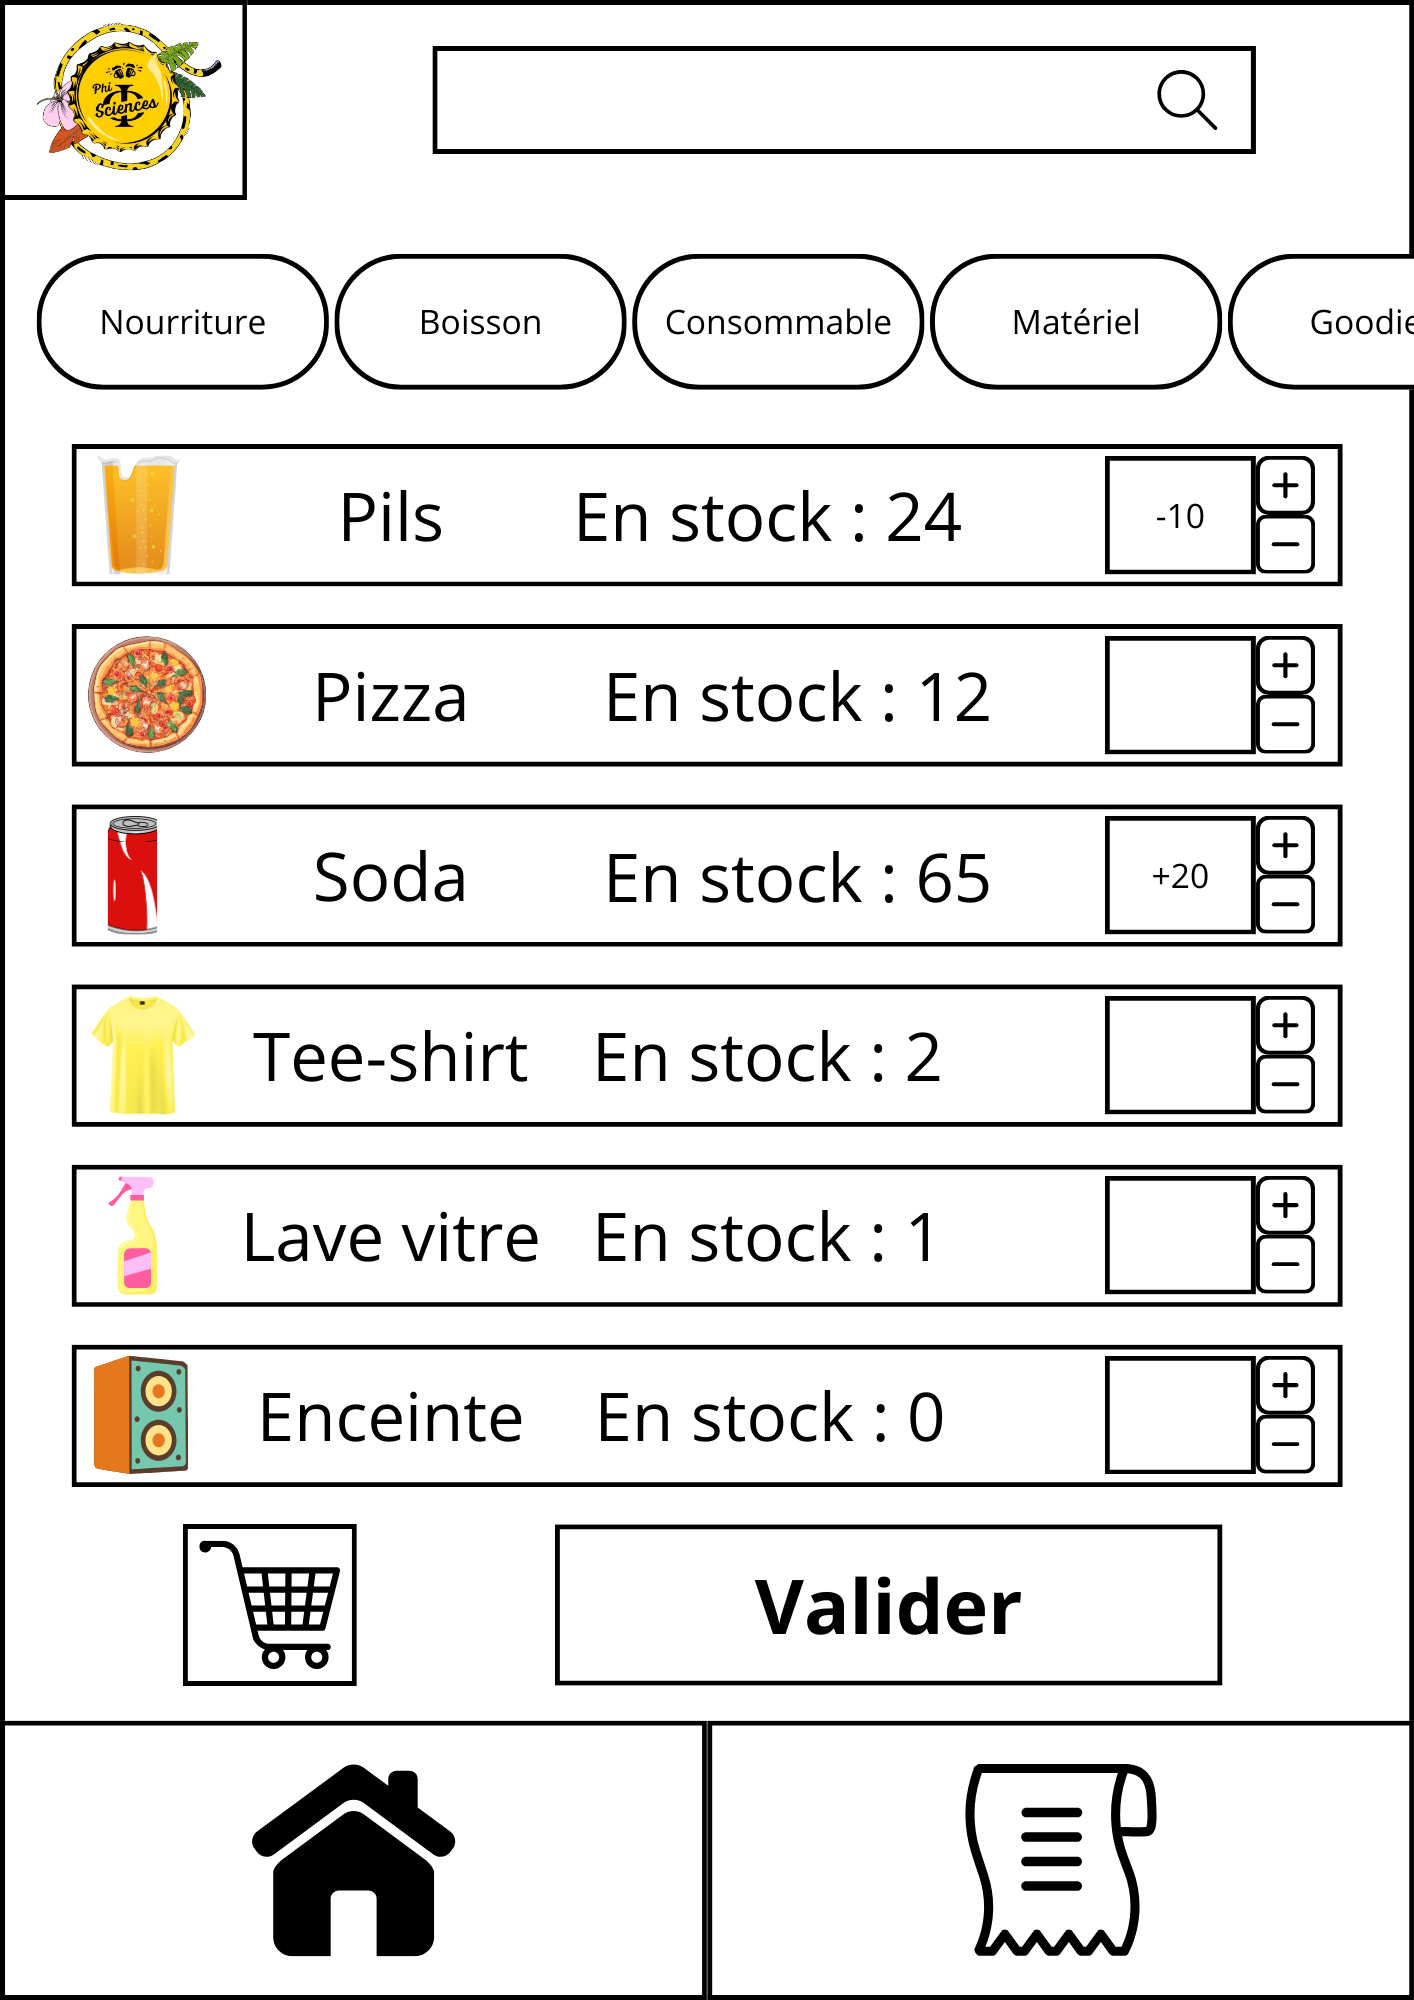
\includegraphics[width=0.8\linewidth]{../cachier des charges/Maquette_appli/Home_page.png} 
    \caption{Maquette}
    \label{fig:maquette}
\end{wrapfigure}
Une fois la totalité des cas d'utilisations énumérés et réfléchis, je me suis attelé à effectuer plusieurs maquettes de l'application pour que le CA puisse visualiser l'aspect général qu'aurait l'application et me faire leurs retours.\\
Une fois ces maquettes dessinées et approuvées, elles ont pû rejoindre le reste du cahier des charges, intégralement écrit en langages \LaTeX, afin de le compléter et le faire valider une dernière fois par l'association.
\vspace*{0.2cm}\\
Le cahier des charges maintenant complété et validé, je me suis attelé à la conception de l'application avant de me lancer dans le code.\\
J'ai donc commencé à réfléchir à la structure que j'allais pouvoir donner aux aspects plus techniques du code.\\
Je me suis donc concentré sur deux points en particuliers :
\vspace*{0.3cm}\\
{\large\textbf{La structure de la base de données}}
Tout d'abord, je me suis concentré sur comment stocker l'ensemble des informations entrées dans l'application.\\
Pour cela, je me suis penché sur les différentes données qu'on pourrait entrer dans l'application, leurs informations importantes et leurs liens entre elles.
\vspace*{0.2cm}\\
Grâce à lapplication Looping\cite{Looping}, j'ai donc créé le \hyperref[fig:modele]{Modèle de données} de la façon suivante :
j'ai d'abord créé les 4 entités \textbf{Alimentaire}, \textbf{Consommable}, \textbf{Matériel} et \textbf{Goodies}.\\
J'ai ensuite associé à l'entité \textbf{matériel} les deux entités \textbf{Utilisation} et \textbf{Prêt}. 
Chaque Matériel peut avoir été prêté ou utilisé entre 0 et n fois et chaque utilisation ou prêt concerne entre 1 et n matériels.
\vspace*{0.2cm}\\
J'ai remarqué que tous les objets du stock avait des attributs en commun, j'ai donc décidé de les regrouper sous une même super catgéorie, l'entité Item.
\vspace*{0.2cm}\\
Ensuite, j'ai ajouté le fait que des paniers puissent être crée pour que l'utilisateur puisse modifier les quantités de plusieurs objets en même temps.
Ainsi, chaque panier peut contenir plusieurs items et chaque item peut être contenu par plusieurs paniers en même temps.
\vspace*{0.2cm}\\
Enfin j'ai ajouté l'entité \textbf{Serveur} et \textbf{Historique} avec leurs relations correspondantes :
Un panier/historique appartient à un seul et unique serveur et chaque serveur a 0 ou 1 panier/historique. 
\vspace*{0.3cm}\\
{\large\textbf{La structure des classes de mon code }} Concernant la création des classes dans mon code, je me suis appuyé sur mon modèle de base de données.\\
J'ai donc assez facilement créer sur le site Plant UML\cite{Plant} un \hyperref[fig:modele]{Diagramme de classes} très similaire au modèle de données.
\newpage
\phantomsection\label{fig:modele}
\begin{figure}[ht]

    \begin{subfigure}{0.5\textwidth}
    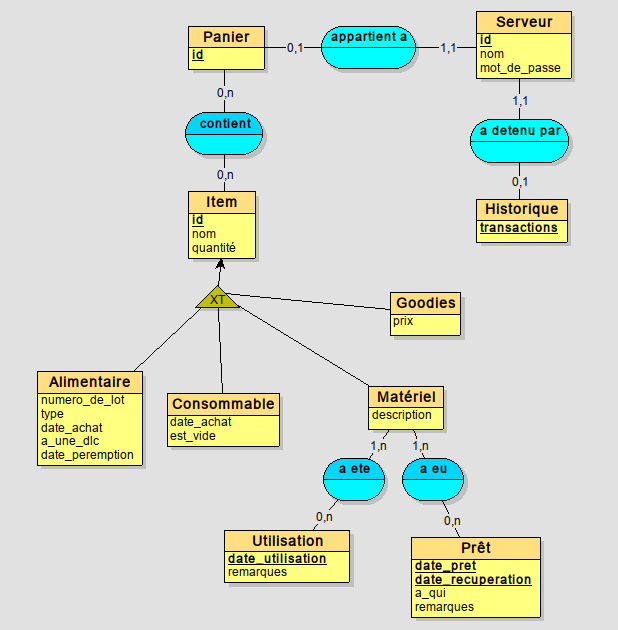
\includegraphics[width=0.9\linewidth, height=6cm]{modele.png} 
    \caption{Modele de données}
    \label{fig:subim1}
    \end{subfigure}
    \begin{subfigure}{0.5\textwidth}
    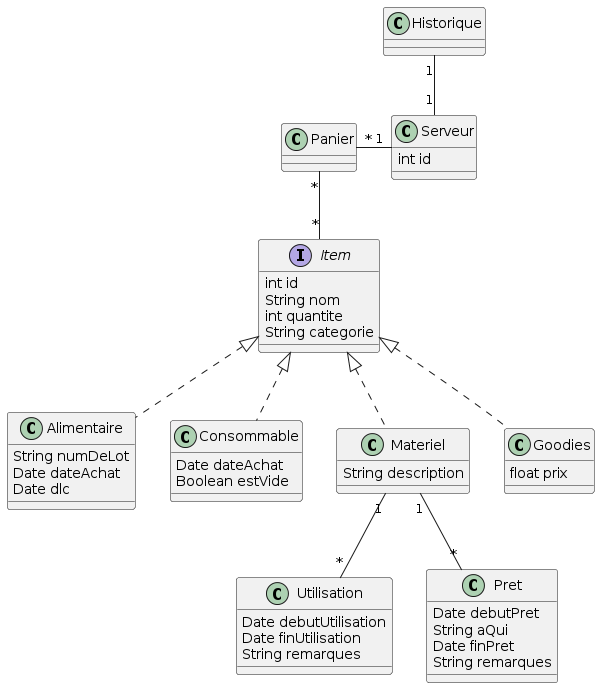
\includegraphics[width=0.9\linewidth, height=6cm]{UML.png}
    \caption{Diagramme de classes}
    \label{fig:subim2}
    \end{subfigure}
    
    \label{fig:image2}
\end{figure}
Une fois ces deux schémas construits, j'ai pû commencer à me lancer dans l'écriture du code de l'application.
\vspace*{0.2cm}\\
Ayant déjà la structure globale de la base de données et du modèle de classe, j'ai décidé de commencer par coder ces deux aspects avant de créer l'interface utilisateur.
Tout d'abord, concernant la base de données, j'ai décidé d'utiliser \underline{SQLite}\cite{Sql}, langage avec lequel je suis très familier, l'ayant utilisé pendant l'intégralité de ma licence.
\vspace*{0.2cm}\\
Une fois la base de données mise en place, je me suis lancé dans l'écriture de mes classes. 
Pour cela, j'ai décidé de coder l'application en Java\cite{Java} sous Android Studio\cite{AndroidStudio}. \\
J'ai fait ce choix car d'une part j'étais déjà familiarisé avec ce langage et cet environnement et d'autre part car le délai pour coder l'application devenant assez court, je ne pensais pas avoir le temps de redécouvrir un nouveau langage ou un nouvel environnement. \\
J'ai aussi choisi l'environnement Android Studio\cite{AndroidStudio} plutôt qu'un autre afin de faciliter la création de l'interface utilisateur par la suite.\\
En effet, il contient une fonctionnalité (scene builder) qui facilite grandement la création de FXML pour la création des différentes scènes de l'interface.
\vspace*{0.2cm}\\
J'ai donc par la suite codé l'intégralité des classes en suivant le Diagramme de classe que j'avais précédemment établi et en veillant bien à effectuer des tests JUnit pour chaque fonctionnalité que j'implémentais.
\vspace*{0.2cm}\\
Après avoir codé le modèle explicité ci-dessus, j'ai essayé de mettre en place le stockage de l'historique sour forme de JSON.\\
En effet, les modifications du stock pouvant survenir plusieurs fois par jours et par bénévole, il est primordiale de trouver un moyen de stocker l'historique qui n'utilise pas trop d'espace ou de mémoire.\\
Malheureusement, j'ai rencontré quelques soucis sur la gestion de ses fichiers au niveau de l'écriture et de la lecture mais surtout au niveau de leur stockage dans la base de donnée.\\
J'ai donc décidé de laisser de côté cette fonctionnalité pour faire mon mieux pour rendre l'application utilisable. 
Faute de temps, je n'ai pas pu, au final, revenir sur cette fonctionnalité pour essayer de la corriger.
\vspace*{0.2cm}\\
Une fois le modèle opérationnel, et après avoir vérifié que les autres actions possibles par l'utilisateur ont bien été implémentées, je me suis lancé dans la création de l'interface en utilisant Scene Builder et des Controllers afin de relier l'interface aux fonctionnalités que je venais de construire.

\subsection{Etat actuel du travail}
À l'issu de ces deux mois de stage, l'application est fonctionnelle et elle peut être utilisée par plusieurs membres actifs de l'association en simultané.\\
Seuls les historiques des bénévoles ne sont pas sauvegardés. 
Ils peuvent intéragir avec la base de donnée mais la trace de ces modifications ne peuvent pas être vérifié dans l'application.
\vspace*{0.2cm}\\
À part concernant le point ci-dessus, le planning et les objectifs que nous nous étions fixés avec M. Louis Maire en début de stage ont été atteint.
Il manquera uniquement quelques retouches pour pouvoir retransmettre l'application à d'autres associations, si elles le souhaitent et valider les objectifs qui se sont ajoutés en cours de stage.\\
Une fois ces points rectifiés, l'application pourra être utilisée par l'ensemble de l'équipe de Phi-Sciences dès la rentrée scolaire 2024 et peut déjà être installée sur les appareils de ceux souhaitant la découvrir avant ce moment.
\vspace*{0.2cm}\\
L'association va se mettre à la recherche d'autres développeurs afin de pouvoir commencer à travailler sur l'application de gestion de vente qui sera raccrochée à celle que j'ai pû leur créer.
\newpage

\section{Conclusion}
Pour conclure ce rapport de stage, je vais décrire ce stage de trois points de vue différents.\vspace*{0.2cm}\\
Je vais d'abord en faire un bilan en explicitant les différentes difficultés que j'ai pû rencontrer mais aussi faire un point sur l'avancée globale du projet.\\
Ensuite, je mettrais en relation ce stage avec les compétences que j'ai pû acquérir ou non lors de ma formation universitaire.\\
Enfin, je parlerais de mon ressenti vis-à-vis de ce stage en appuyant sur les éléments de réussites ou les difficultés que j'ai pû surmonter durant ces 2 mois.
\vspace*{0.3cm}\\
Tout d'abord, commençont par faire un point sur \textbf{l'avancée globale du projet}.
\vspace*{0.2cm}\\
L'objectif de ce stage était d'effectuer un cahier des charges et coder une application mobile permettant aux membres actifs de Phi-Sciences de gérer les stocks de l'association.
Sachant que l'accessibilité et la facilité de prise en main étaient des points très importants de ce stage.
\vspace*{0.2cm}\\
Au cours de ces 2 mois, un autre objectif a été relevé : Faire en sorte que l'application soit personnalisable afin que d'autres associations puissent en profiter.
\vspace*{0.2cm}\\
Au bout de ce stage, le cahier des charges a été complétement rédigé et validé par le Conseil d'Administration de l'association et l'application peut dores et déjà être téléchargée et utilisée par tous les membres de Phi-Sciences.\\
En plus de cela, les différents tutoriels expliquant la maintenance de l'application et son utilisation ont eux aussi été rédigés en tenant compte du niveau de connaissances en informatique des membres de l'association.
\vspace*{0.2cm}\\
Enfin, par manque de temps, la sauvegarde et l'affichage des historiques des utilisateurs ainsi que la personnalisation de l'application n'ont pas pû être correctement implémentés.\\
J'ai préféré, après discussion avec mon maître de stage, prioriser la conception même de l'application et le fait qu'elle fonctionne pour les membres de Phi-Sciences avant de me concentrer sur la personnalisation.
\vspace*{0.2cm}\\
Ainsi, il ne resterait plus qu'à implémenter le changement de charte graphique (couleur de fond et des boutons) pour que tous les objectifs déterminés au cours du stage soient complétés.
\vspace*{0.3cm}\\
Ensuite, je vais au mieux faire le \textbf{lien entre les compétences qui m'étaientt nécessaires pour mener à bien mon stage et celles que j'ai pû acquérir au cours de mon parcours étudiant}.
\vspace*{0.2cm}\\
Dans un premier temps, analysons les compétences qui m'ont servi à établir le cahier des charges.
\vspace*{0.2cm}\\
Il est vrai que la grande majorité de mes connaissances sur les cahiers des charges viennent de l'UE Conception Programmation Objet Avanceée (CPOA) qui visait principalement à nous apprendre les outils et les méthodes pour rédiger un cahier des charges.\\
Ce cours m'a permis de savoir efficacement comment retransmettre et traduire les fonctionnalités de l'application à des personnes n'ayant pas forcément de compétences en informatique.
\vspace*{0.2cm}\\
Dans un second temps, si nous analysons la programmation même de l'application nous pouvons remarquer que la totalité des outils utilisés sont des outils présentés et utilisés durant les différentes UE de ma licences.\\
En effet, plantUML était extrêmement utilisé lors des cours de programmation en java, Looping me vient des cours de Base De Données et Android studio était l'environnement préconisé dans l'UE Développement Mobile.\\
Cette dernière UE m'a d'ailleurs apporté beaucoup de connaissances qui m'ont été fortement utile au bon déroulé du stage, ce dernier ayant pour sujet la création d'une application mobile.
\vspace*{0.2cm}\\
Pendant ces 2 mois, j'ai ressenti que je pouvais piocher dans mon expérience de ces 3 dernières années assez facilement pour les appliquer dans un contexte autre que celui des cours.
L'un des principaux moment où j'ai ressenti un manque de connaissance était quand j'étais confronté au problèmes liés aux JSON (écriture, lecture et stockage).
\vspace*{0.3cm}\\
Enfin, je vais finir ce rapport et cette conclusion sur une touche plus personnelle en faisant un \textbf{bilan parlant des points de satisfaction et les difficultés que j'ai pu rencontrer et surmonter}.
\vspace*{0.2cm}\\
Tout d'abord je suis assez satisfait du travail que j'ai pu accomplir dans ce délai assez court en partant de 0.
\vspace*{0.2cm}\\
Ensuite, je trouve qu'il est vraiment récompensant de voir que les compétences que l'ont peut acquérir tout au long de notre licence sont facilement réutilisables dans des cas plus concrets.
\vspace*{0.2cm}\\
Enfin, pour parler des difficultés que j'ai pu rencontrer, l'une des plus grosses à laquelle je me suis heurté est le temps. \\
Un stage de 2 mois est au final très court et passe bien plus vite qu'on ne le pense et j'aurais aimé pouvoir finir de mettre en place les dernières fonctionnalités manquantes. 
Je reste tout de même fier du travail que j'ai pu accomplir durant ces 2 mois pour cette association.
\newpage

\section{Bibliographie}
\printbibliography

\end{document}